\documentclass[a4paper, amsfonts, amssymb, amsmath, reprint, showkeys, showpacs, nofootinbib, twoside]{revtex4-2}
\usepackage[english]{babel}
\usepackage[utf8]{inputenc}
\usepackage[colorinlistoftodos, color=green!40, prependcaption]{todonotes}
\usepackage{bm}% bold math
\usepackage{amsthm}
\usepackage{mathtools}
\usepackage{physics}
\usepackage{xcolor}
\usepackage{graphicx}
\usepackage[left=23mm,right=13mm,top=35mm,columnsep=15pt]{geometry} 
\usepackage{adjustbox}
\usepackage{placeins}
\usepackage[T1]{fontenc}
\usepackage{lipsum}
\usepackage{csquotes}
\usepackage[pdftex, pdftitle={Article}, pdfauthor={Author}]{hyperref} % For hyperlinks in the PDF
%\setlength{\marginparwidth}{2.5cm}
\bibliographystyle{apsrev4-2}
\hypersetup{
    colorlinks=true,     % 使用彩色链接
    linkcolor=blue,      % 设置内部链接的颜色
    citecolor=blue,      % 设置引用的颜色
    urlcolor=blue        % 设置网址的颜色
}

\begin{document}
\title{Collective Behavior, Chemotaxis and Chirality in Active Matter: A Review
}

\author{Yichen Lu$^{1,2}$}
\author{Zhigang Zheng$^{1,3}$}
\email{Corresponding author. zgzheng@hqu.edu.cn}

\affiliation{ 
$^1$Institute of Systems Science, Huaqiao University, Xiamen 361021, China\\
$^2$School of Mathematical Sciences, Huaqiao University, Quanzhou, 362021, China\\
$^3$College of Information Science and Technology, Huaqiao University, Xiamen 361021, China
}

\date{\today} % Leave empty to omit a date

\begin{abstract}
    Active matter refers to a class of systems composed of self-propelled particles that can convert energy into motion and exhibit a variety of collective behaviors, such as flocking, swarming, and clustering. In this review, we focus on the collective behaviors of active matter, with a particular emphasis on the role of chemotaxis and chirality in shaping these behaviors. Chemotaxis is the ability of cells or organisms to move in response to chemical gradients in their environment, and it plays a crucial role in many biological processes, such as wound healing, immune response, and cancer metastasis. Chirality refers to the property of an object that is not superimposable on its mirror image, and it is a common feature of many biological systems, such as DNA, proteins, and cells. The combination of chemotaxis and chirality can lead to a wide range of interesting collective behaviors in active matter, such as phase separation, pattern formation, and dynamic self-assembly. We introduce the Keller--Segel and phoretic Brownian particle models of chemotactic active matter and discuss the role of chemotaxis in shaping the collective behaviors of active particles. We present the chiral active particle model and its extension and discuss the role of chirality in shaping the collective behaviors of active particles. Furthermore, we summarize the main findings of the review and discuss future research directions in the field of active matter.
\end{abstract}

\pacs{pacs}  % PACS, the Physics and Astronomy  % Classification Scheme.
\keywords{active matter, chemotaxis, chirality, collective behavior}

\maketitle

\section{\label{sec:introduction}Introduction}

We live in a colorful world filled with numerous systems composed of various different individuals, and these systems exhibit a wide range of collective behaviors. For example, we can directly observe many interesting behaviors of biological groups, such as the dynamic collective flight of flocks of birds, the complex collective swimming of schools of fish, the busy and orderly collective activities of large ant colonies, and the collective flashing of countless fireflies at night in tropical regions. These collective behaviors are not only fascinating but also have important implications for the survival and evolution of these groups. In recent years, the study of collective behaviors has become a hot topic in the field of complex systems, and the development of active matter theory has provided a new perspective for understanding these phenomena \cite{Liebchen_2022,Liebchen_2018,PhysRevLett.127.238001,Ziepke2022,PhysRevLett.118.268001,PhysRevLett.119.058002,LU2025115794}.

Active matter refers to a class of systems composed of self-propelled particles that can convert energy into motion and exhibit a variety of collective behaviors, such as flocking, swarming, and clustering. The study of active matter has attracted the attention of many researchers from different fields, including physics, biology, and engineering, and has led to the development of a new interdisciplinary research field. The collective behaviors of active matter are not only interesting from a fundamental scientific perspective but also have important applications in various fields, such as robotics, materials science, and drug delivery.

In this review, we focus on the collective behaviors of active matter, with a particular emphasis on the role of chemotaxis and chirality in shaping these behaviors. Chemotaxis is the ability of cells or organisms to move in response to chemical gradients in their environment, and it plays a crucial role in many biological processes, such as wound healing, immune response, and cancer metastasis. Chirality refers to the property of an object that is not superimposable on its mirror image, and it is a common feature of many biological systems, such as DNA, proteins, and cells. The combination of chemotaxis and chirality can lead to a wide range of interesting collective behaviors in active matter, such as phase separation, pattern formation, and dynamic self-assembly.

The review is organized as follows. In Section~\ref{sec:models}, we introduce the Keller--Segel and phoretic Brownian particle models of chemotactic active matter and discuss the role of chemotaxis in shaping the collective behaviors of active particles. In Section~\ref{sec:chirality}, we present the chiral active particle model and its extension, and we discuss the role of chirality in shaping the collective behaviors of active particles. In Section~\ref{sec:conclusions}, we summarize the main findings of the review and discuss future research directions in the field of active matter.

\begin{figure*}
    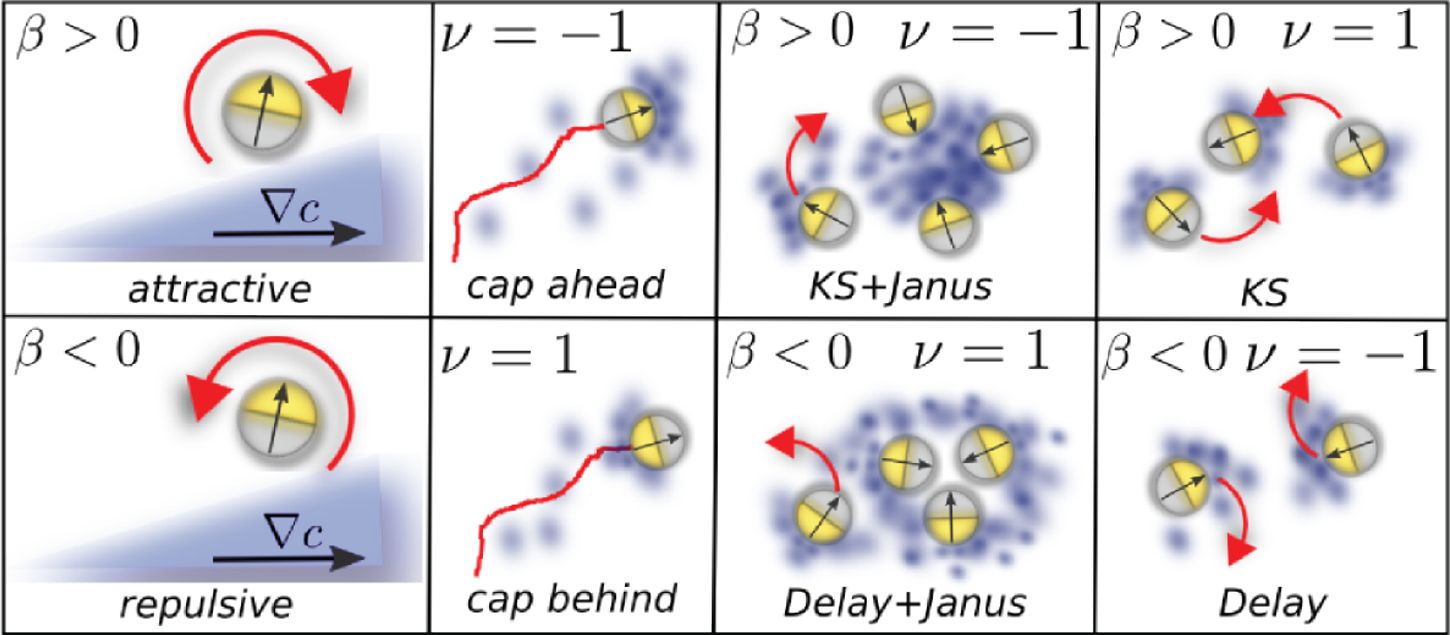
\includegraphics[width=0.7\textwidth]{./figs/schematicPlot1.png}
    \caption{
        \label{fig:schematicPlot1} Schematic plot of the chemotactic response of active particles to a chemo-attractant. Here, KS represents the Keller--Segel instability, and Janus and Delay stand for the Janus instability and the delay induced instability discussed in the text. Reproduced with permission from ref.~\cite{PhysRevLett.118.268001}. Copyright 2017 American Physical Society.
    }
\end{figure*}

\section{\label{sec:models}Models of Chemotactic Active Matter}

\subsection{The Keller--Segel And Phoretic Brownian Particle Models}
The mechanism of chemotaxis is captured in the classical Keller--Segel model and has recently been established also for E. coli bacteria showing positive chemotaxis to self-produced autoinducers. The Langevin equation model of agent-based model is defined as
\begin{subequations}
    \label{eq:agentsChemotaxis}
    \begin{align}
        &\dot{\mathbf{r}}_i(t)=\beta_D\nabla c(\mathbf{r}_1(t),t)+\sqrt{2D}\boldsymbol{\xi }(t)\;,\\
        &\dot{c}(\mathbf{r},t)=D_c\Delta c(\mathbf{r},t)+k_0\delta (\mathbf{r}-\mathbf{r}_i)-k_dc(\mathbf{r},t)\;,
    \end{align}
\end{subequations}
where $\mathbf{r}_i$ is the position of the $i$th particle, $c(\mathbf{r},t)$ is the concentration of the chemo-attractant, $\beta_D$ is the chemotactic sensitivity, which is a key parameter that determines the strength of the chemotactic response of the particles to the chemo-attractant. The chemotactic sensitivity can be positive or negative, depending on the nature of the chemo-attractant. If the chemo-attractant is attractive, the chemotactic sensitivity is positive, and the particles move toward regions of higher chemo-attractant concentration. If the chemo-attractant is repulsive, the chemotactic sensitivity is negative, and the particles move away from regions of higher chemo-attractant concentration, as shown in Fig.~\ref{fig:schematicPlot1}.
Here, $D$ is the translational diffusion coefficient, $D_c$ is the diffusion coefficient of the chemo-attractant, $k_0$ is the rate of chemo-attractant production, $k_d$ is the rate of chemo-attractant degradation, and $\boldsymbol{\xi }(t)$ is a Gaussian white noise with zero mean and unit variance.

Based on the hydrodynamic theory, the macroscopic equations for the system in Eqs.~\eqref{eq:agentsChemotaxis} with the density $\rho (\mathbf{r},t)$ and the concentration $c(\mathbf{r},t)$ of the chemo-attractant are given by
\begin{subequations}
    \label{eq:hydroChemotaxis}
    \begin{align}
        &\dot{\rho}\left( \mathbf{r},t \right) =-\nabla \cdot \left( \beta _D\rho \left( \mathbf{r},t \right) \nabla c\left( \mathbf{r},t \right) \right) +D\nabla ^2\rho \left( \mathbf{r},t \right)\\
        &\dot{c}\left( \mathbf{r},t \right) =D_c\nabla ^2c\left( \mathbf{r},t \right) +k_0\rho \left( \mathbf{r},t \right) -k_dc\left( \mathbf{r},t \right)\;.
    \end{align}
\end{subequations}
These equations represent the classical Keller--Segel model. The chemotactic sensitivity $\beta _D$ is a key parameter that determines the strength of the chemotactic response of the particles to the chemo-attractant. The chemotactic sensitivity can be positive or negative, depending on the nature of the chemo-attractant. If the chemo-attractant is attractive, the chemotactic sensitivity is positive, and the particles move toward regions of higher chemo-attractant concentration. If the chemo-attractant is repulsive, the chemotactic sensitivity is negative, and the particles move away from regions of higher chemo-attractant concentration.

One obvious solution of Eqs.~\eqref{eq:hydroChemotaxis} is $(\rho, c)=(\rho_0, k_0\rho_0/k)$ representing a uniform disordered phase. Performing a linear stability analysis of this phase predicts a criterion for the onset of structure formation, which reads:
\begin{equation}
    \label{eq:KSinstability}
    k_0\rho_0\beta_D>D k_d\;.
\end{equation}
This is the Keller--Segel instability, which occurs for chemoattraction ($\beta_D>0$) and a sufficiently high chemoattractant production rate $k_0$. The instability leads to the formation of spatial structures in the density field $\rho(\mathbf{r},t)$ and the chemo-attractant concentration field $c(\mathbf{r},t)$, as shown in Fig.~\ref{fig:schematicPlot1}.

\begin{figure*}
    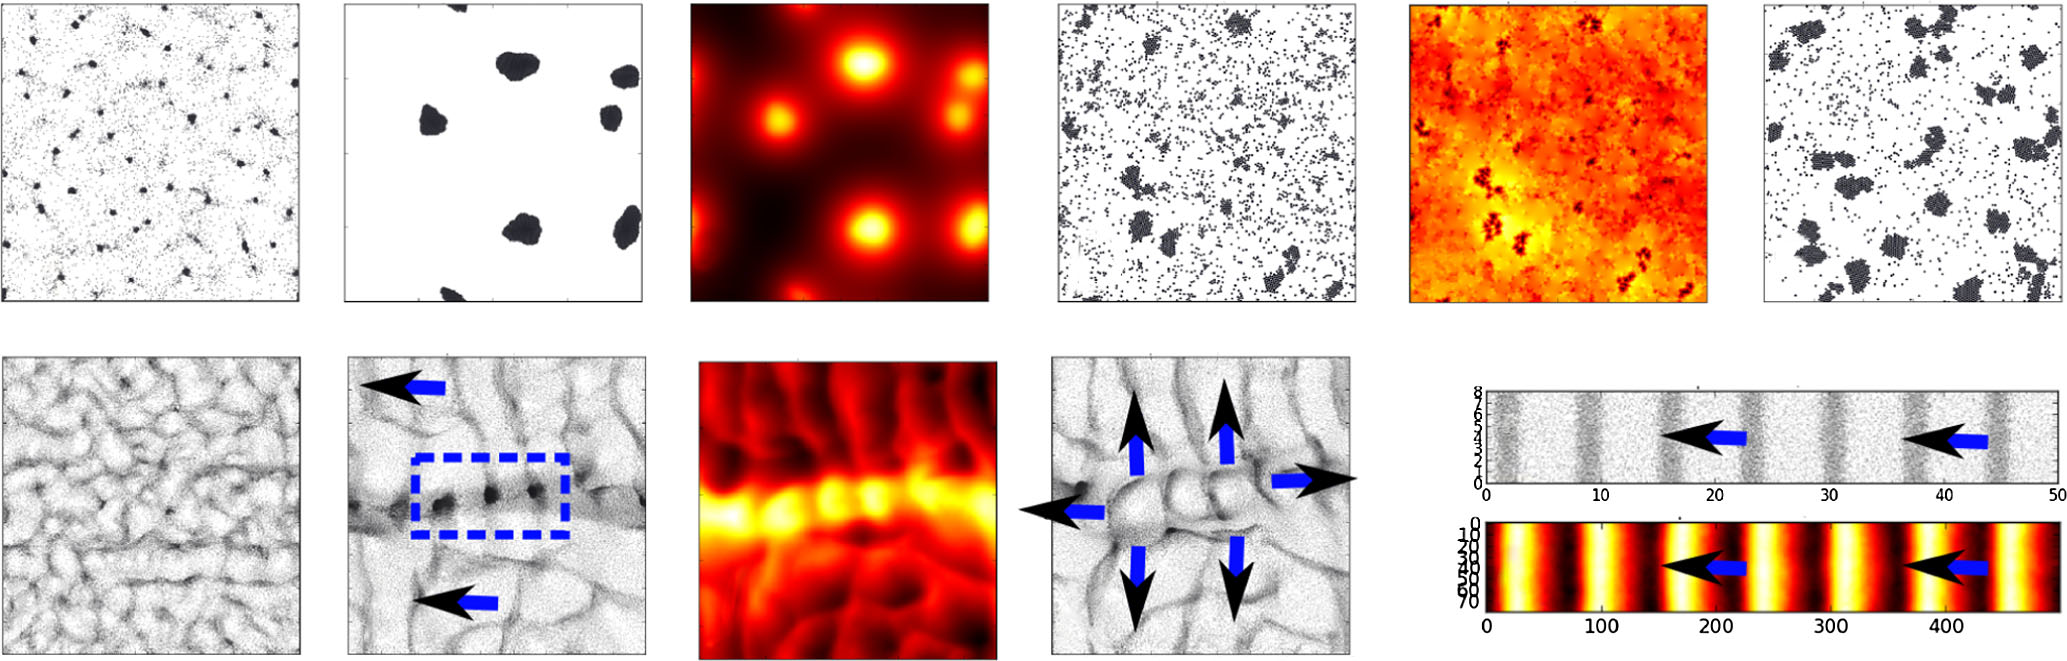
\includegraphics[width=\textwidth]{./figs/chemoBehaviors1.png}
    \caption{
        \label{fig:chemoBehaviors1} Generic patterns in phoretic Janus colloids: snapshots from agent-based simulations.
        Reproduced with permission from ref.~\cite{PhysRevLett.118.268001}. Copyright 2017 American Physical Society.
    }
\end{figure*}

When subjected to a chemical gradient, anisotropic particles—like self-propelled Janus colloids—can experience both displacement (a change in velocity) and alignment with or against the gradient (a change in self-propulsion direction). Essentially, this means they are influenced by both a force acting on their center of mass and a torque. The dynamics of such particles can be described by the motion of an overdamped chemotactic particle self-propelling with a velocity $v_0$ (independently of chemotaxis) in a direction $\mathbf{p}=\left(\cos\theta, \sin\theta\right)$ in two dimensions by the following evolution equations \cite{PhysRevLett.118.268001}
\begin{subequations}
    \label{eq:JanusChemotaxis}
    \begin{align}
        &\dot{\mathbf{r}}_i(t)=v_0\mathbf{p}_i\;,\\
        &\dot{\theta}_i(t)=\beta \mathbf{p}_i\times \nabla c(\mathbf{r}_i)+\sqrt{2D_{\mathbf{r}}}\xi _i(t)\;,\\
        &\dot{c}(\mathbf{r},t)=D_c\nabla ^2c(\mathbf{r},t)-k_dc(\mathbf{r},t)\notag\\
        &+\sum_{i=1}^N{\oint{\mathrm{d}\mathbf{x}_i\delta \left(\mathbf{r}-\mathbf{r}_i(t)-R_0\mathbf{x}_i\right)\sigma (\mathbf{x}_i)}}\;.
    \end{align}
\end{subequations}
The underlying physical mechanism is illustrated in Fig.~\ref{fig:chemoBehaviors1}. 

To understand the collective behavior of agents-based model Eqs.~\eqref{eq:JanusChemotaxis}, Liebchen et al. coarse-grained the model and derived the following hydrodynamic equations
\begin{subequations}
    \label{eq:hydroJanusChemotaxis}
    \begin{align}
        \dot{\rho}&=-\mathrm{Pe}\nabla \cdot \mathbf{w},\\
        \dot{\mathbf{w}}&=-\mathbf{w}+\frac{B\rho}{2}\nabla c-\frac{\mathrm{Pe}}{2}\nabla \rho +\frac{\mathrm{Pe}^2}{16}\nabla ^2\mathbf{w}-\frac{B^2|\nabla c|^2}{8}\mathbf{w}\notag\\
        &+\frac{\mathrm{Pe}B}{16}[3(\nabla \mathbf{w})^T\cdot \nabla c-(\nabla c\cdot \nabla )\mathbf{w}-3(\nabla \cdot \mathbf{w})\nabla c],\\
        \dot{c}&=\mathcal{D} \nabla ^2c+K_0\rho +\boldsymbol{\nu }\frac{K_0}{2}\nabla \cdot \mathbf{w}-K_dc.\label{eq:hydroJanusChemotaxis2}
    \end{align}
\end{subequations}
One limiting case of Eqs.~\eqref{eq:hydroJanusChemotaxis} is the Keller--Segel instability, which is obtained for quasi-instantaneous alignment of the particles to the chemical gradients ($\mathbf{w}\rightarrow 0$) when neglecting the nonlinearity and second-order gradients in the equation for Eq.~\eqref{eq:hydroJanusChemotaxis2}, that is, $\mathbf{w}\sim B\rho\nabla c/2-\mathrm{Pe}\nabla\rho/2$. Plugging this expression into Eq.~\eqref{eq:hydroJanusChemotaxis2} yields the Keller--Segel instability criterion for $\nu=0$. Therefore, the formal analogy of Keller--Segel allows for the identification of the Janus instability as
\begin{equation}
    \label{eq:JanusInstability}
    \frac{K_0\rho_0 B}{K_d\mathrm{Pe}}>1\;.
\end{equation} 
The Janus instability leads to the formation of spatial structures in the density field $\rho(\mathbf{r},t)$ and the chemo-attractant concentration field $c(\mathbf{r},t)$, as shown in Fig.~\ref{fig:chemoBehaviors1}.

\subsection{The Communicating Active Matter Model}
To reveal the fundamental role of interparticle communication for self-organization, Ziepke et al. \cite{Ziepke2022} introduced a system of self-propelled units (agents) with local polar-alignment interactions and chemotactic coupling to a common chemical field. The model is described by the following equations
\begin{subequations}
    \label{eq:communicatingActiveMatter}
    \begin{align}
        &\dot{\mathbf{r}}_i=v_0\mathbf{n}_i+\sum_{j\left[ r_{ij}<2r_p \right]}{f_{ij}}\;,\\
        &\dot{\varphi}_i=-\varGamma \sum_{j\left[ r_{ij}<r_c \right]}{\frac{\sin \left( \varphi _i-\varphi _j \right)}{\left| \mathbf{r}_i-\mathbf{r}_j \right|}}+\omega \sin \left( \varphi _c-\varphi _i \right) +\xi _i\;,\\
        &\dot{c}\left( \mathbf{r},t \right) =D_c\Delta c-\alpha c+\beta \sum_{i=1}^N{f\left( \left| \mathbf{r}-\mathbf{r}_i \right| \right) \phi \left( s_i,c \right)}\;,\\
        &\dot{s}_i=\epsilon \left( c-s_i \right)\;,
    \end{align}
\end{subequations}
where $\mathbf{r}_i$, $\varphi _i$ and $s_i$ are the position, orientation and internal state of the $i$th particle, respectively. The particles move with a constant speed $v_0$ in the direction of their orientation $\mathbf{n}_i=\left( \cos \varphi _i,\sin \varphi _i \right)$. The alignment interaction is modeled by a polar alignment force between particles $i$ and $j$ within a distance $2r_c$. The chemotactic coupling is mediated by a chemical field $c(\mathbf{r},t)$, which is produced by the particles and diffuses with a diffusion coefficient $D_c$. The particles respond to the chemical field through a chemotactic function $\phi \left( s_i,c \right)$, which depends on the internal state $s_i$ of the particles. The alignment interaction is mediated by a coupling strength $\varGamma$ and an intrinsic angular velocity $\omega$. The noise term $\xi _i$ is a Gaussian white noise with zero mean and unit variance. The model is illustrated in Fig.~\ref{fig:chemoBehaviors2}.

\begin{figure}
    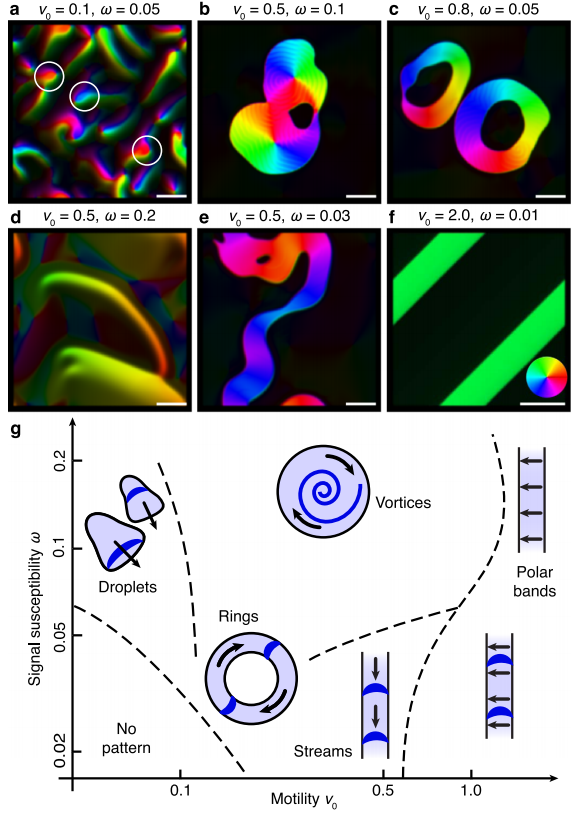
\includegraphics[width=0.49\textwidth]{./figs/chemoBehaviors2.png}
    \caption{
        \label{fig:chemoBehaviors2} Principal collective dynamic states in the hydrodynamic model.
        The phase diagram of dominant (meta-stable) dynamic states in the $\omega-v_0$ (signal susceptibility and motility) parameter space is shown in the lower panel \textbf{g}.
        Reproduced with permission from ref.~\cite{Ziepke2022}. Copyright 2022 Springer Nature.
    }
\end{figure}

\begin{figure*}
    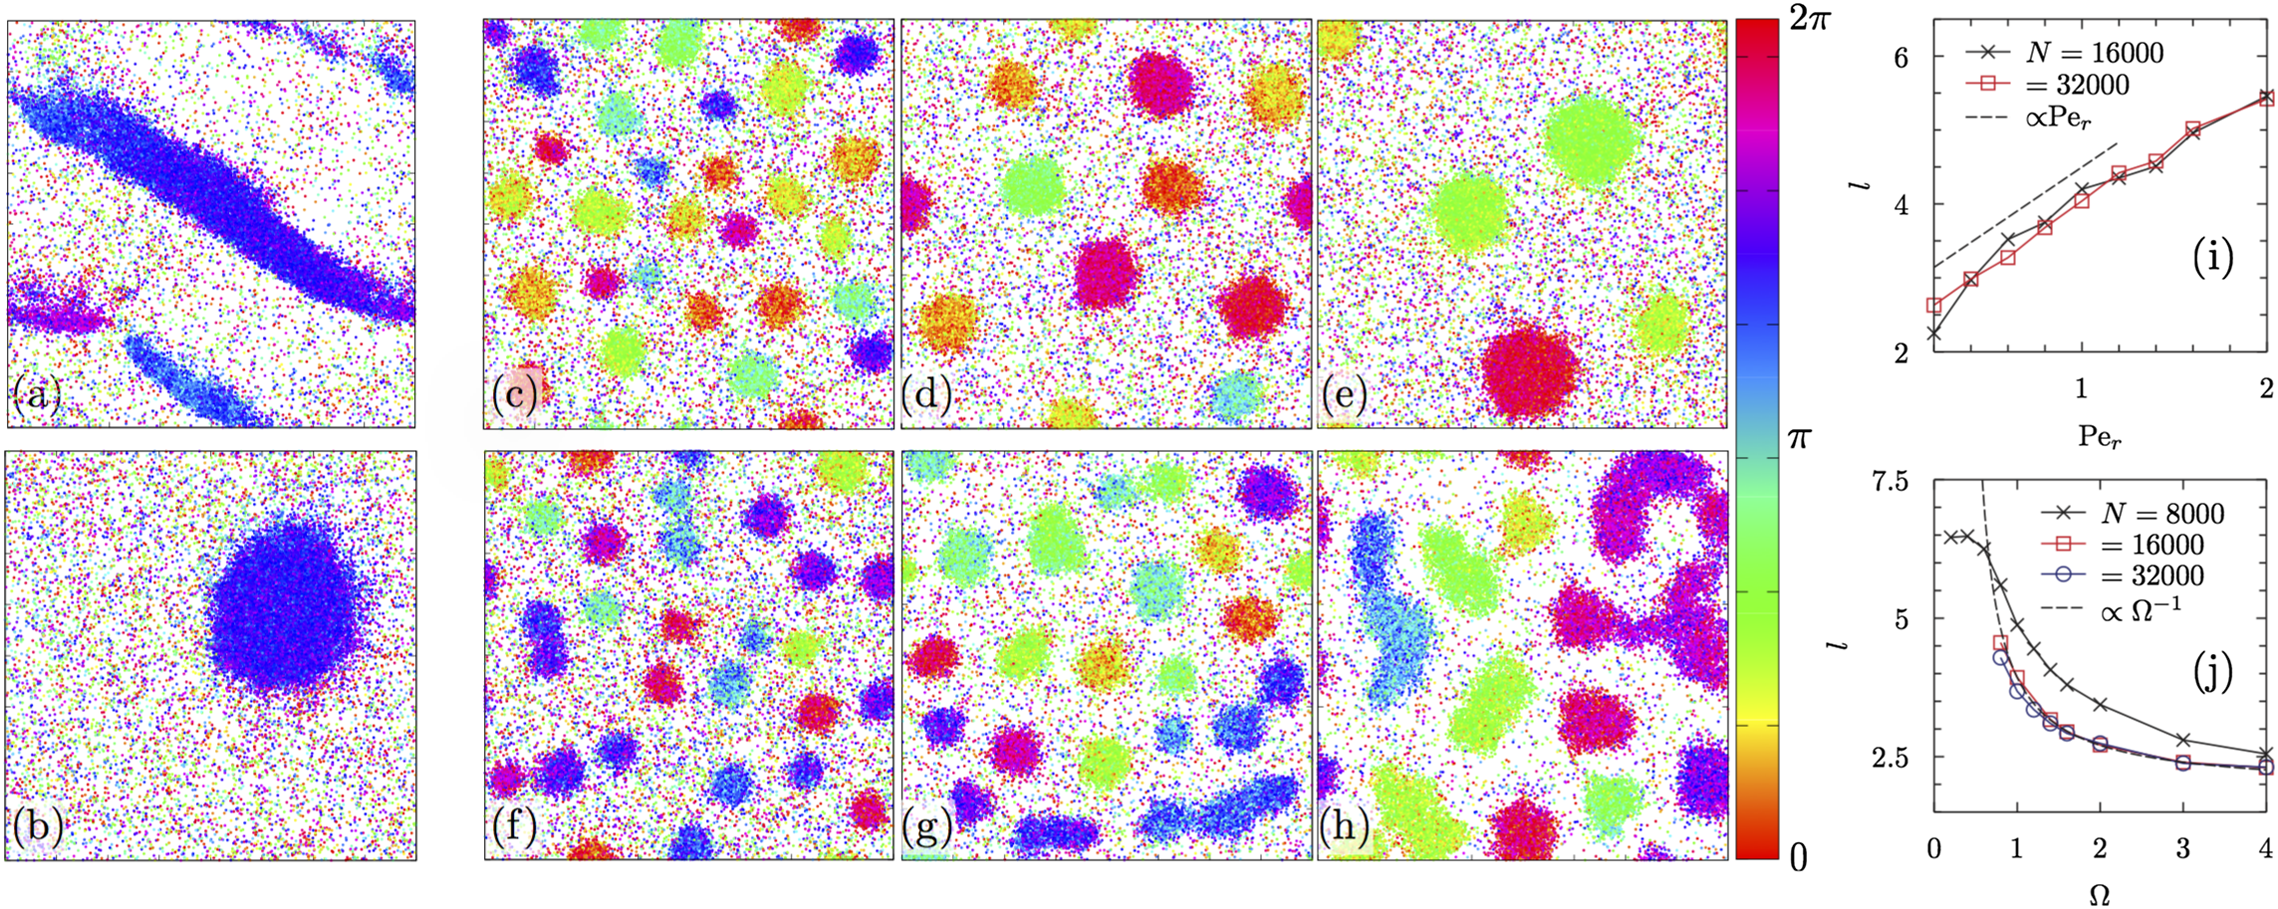
\includegraphics[width=\textwidth]{./figs/capBehaviors1.png}
    \caption{
        \label{fig:capBehaviors1} Generic patterns in phoretic Janus colloids: snapshots from agent-based simulations.
        Reproduced with permission from ref.~\cite{PhysRevLett.118.268001}. Copyright 2017 American Physical Society.
    }
\end{figure*}

Similar to the previous model, the hydrodynamic equations for the system in Eqs.~\eqref{eq:communicatingActiveMatter} with the density $\rho (\mathbf{r},t)$ and the concentration $c(\mathbf{r},t)$ of the chemo-attractant are given by
\begin{subequations}
    \begin{align}
        \dot{\rho}\left( \mathbf{r},t \right) &=-v_0\nabla \cdot \mathbf{p}+D_p\Delta \rho\\
        \dot{\mathbf{p}}\left( \mathbf{r},t \right) &=\sigma \left( \rho -1 \right) \mathbf{p}-\delta \left| \mathbf{p} \right|^2\mathbf{p}+D_p\Delta \mathbf{p}\notag\\
        &-\chi \mathbf{p}\cdot \nabla \mathbf{p}-Q\left( \rho \right) \nabla \rho +\rho \omega \nabla c\\
        \dot{c}\left( \mathbf{r},t \right) &=D_c\Delta c-\alpha c+\rho \beta \Theta \left( c-c_{\mathrm{th}} \right) \left( 1-s \right)\\
        \dot{s}\left( \mathbf{r},t \right) &=D_{\rho}\Delta s+\epsilon \left( c-s \right) -\bar{v}\mathbf{p}\cdot \nabla s\;.
    \end{align}
\end{subequations}
The hydrodynamic model consists of a set of coupled partial differential equations governing these fields, utilizing parameters that are largely consistent with those of the agent-based model.

\begin{figure*}
    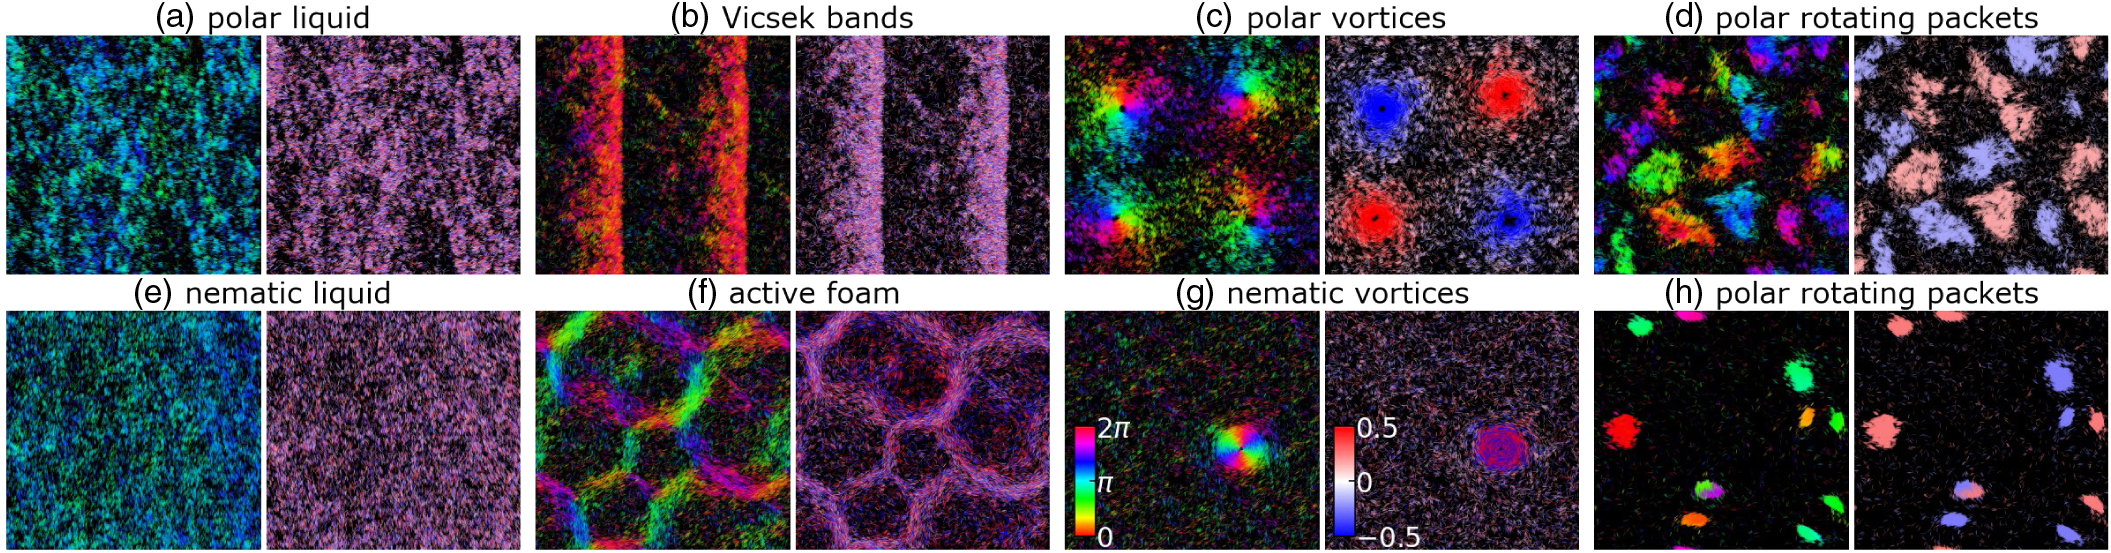
\includegraphics[width=\textwidth]{./figs/capBehaviors2.png}
    \caption{
        \label{fig:capBehaviors2} Typical snapshots of phases of Eqs.~\eqref{eq:CAPextension} taken after transients following random initial conditions.
        Reproduced with permission from ref.~\cite{PhysRevLett.127.238001}. Copyright 2021 American Physical Society.
    }
\end{figure*}

\section{\label{sec:chirality}Models of Chiral Active Matter}
A minimal model describing aligning chiral active matter, originally called the “chiral active particle (CAP) model”, has been introduced in ref. \cite{PhysRevLett.119.058002}. It can be seen as a chiral extension of the classic Vicsek model \cite{PhysRevLett.75.1226}, incorporating additive interactions and operating in continuous time:
\begin{subequations}
    \label{eq:CAP}
    \begin{align}
        \dot{\mathbf{r}}_i&=v_0\mathbf{p}_i,\quad\\
        \dot{\theta}_i&=\omega +\frac{K}{\pi R^2}\sum_{j\in \partial _i}\sin(\theta _j-\theta _i)+\sqrt{2D_R}\eta _i,
    \end{align}
\end{subequations}
where $\mathbf{r}_i$ and $\theta _i$ are the position and orientation of particle $i$, respectively, $v_0$ is the self-propulsion speed, $\omega$ is the intrinsic angular velocity, $K$ is the strength of the alignment interaction, $R$ is the interaction radius, $\partial _i$ denotes the set of particles within the interaction radius of particle $i$, and $\eta _i$ is a Gaussian white noise with zero mean and unit variance. The model is illustrated in Fig.~\ref{fig:capBehaviors1}.

The phenomena described can be broadly analyzed using continuum theories. These theories can be derived through systematic coarse-graining methods, such as Fokker-Planck equations, which are further refined through moment expansions and appropriate closure schemes. For the CAP model Eqs.~\eqref{eq:CAP}, the lowest-order terms in both, gradients and powers of $\mathbf{w}$, read (here written in dimensionless form to simplify the interpretation):
\begin{subequations}
    \begin{align}
        \dot{\rho}&=-\mathrm{Pe}_{\mathrm{r}}\nabla \cdot \mathbf{w},\\
        \dot{\mathbf{w}}&=(g\rho -2)\frac{\mathbf{w}}{2}+\Omega \mathbf{w}_{\bot}-\frac{\mathrm{Pe}_{\mathrm{r}}}{2}\nabla \rho +\mathrm{h}.\mathrm{O}.\;,\label{eq:CAPhydro}
    \end{align}
\end{subequations}
where $\rho$ is the density, $\mathbf{w}$ is the polarization.
The first term on the right-hand side of Eq.~\eqref{eq:CAPhydro} shows that the uniform disordered solution $\left(\rho,\mathbf{w}\right)=\left(\rho_0,\mathbf{0}\right)$ is linearly unstable for $g\rho_0>2$, leading to polarized states. The second term comprises the subscript $\bot$ to denote the perpendicular component of the vector $\mathbf{w}$, which is responsible for the emergence of uniform rotation of aligned particles. The third term represents the relaxation of the polarization field towards the local density gradient, and the last term is higher-order in the gradients and powers of $\mathbf{w}$.

\subsection{The Extension of Chiral Active Particles}
Significantly, reference \cite{PhysRevLett.127.238001} presents a comprehensive analysis of a variant of the CAP model. This variant employs uniform noise and normalizes the interaction term by the local density. The formulation of their model is as follows:
\begin{subequations}
    \label{eq:CAPextension}
    \begin{align}
        &\dot{\mathbf{r}}_i\,\,=\,\,v_0\mathbf{e}(\theta _i),\\
        &\dot{\mathbf{\theta}}_i\,\,=\,\,\omega _i\,\,+\,\,\kappa \langle \sin \alpha (\theta _j-\theta _i)\rangle _{j\sim i}\,\,+\,\,\sqrt{2D_r}\eta _i.\label{eq:CAPextension2}
    \end{align}
\end{subequations}
In particular, this work has identified an additional vortex state, which is also studied by Lu et al. \cite{LU2025115794} and confirmed to be caused by heterogeneity in natural frequencies.
Their work has also explored other (non-ferromagnetic–like) alignment interactions, specifically, it is nematic interactions when $\alpha$ in Eq.~\eqref{eq:CAPextension2} is set to $\alpha =2$, as shown in Fig.~\ref{fig:capBehaviors2}.

Ventejou et al. \cite{PhysRevLett.127.238001} followed the same coarse-graining procedure as in ref. \cite{PhysRevLett.119.058002} to derive the hydrodynamic equations for the CAP model Eqs.~\eqref{eq:CAPextension} and consider the bimodal case (double-chirality) in the following form:
\begin{subequations}
    \begin{align}
        &\partial _t\rho ^+=-\mathrm{Re}[\nabla ^*p],(3\mathfrak{a} )\\
        &\partial _tp=(\mu [\rho ^+,\rho ^-]+i\omega _0-\xi |p|^2)p+\nu \Delta p\notag\\
        &+\kappa _1\nabla ^*p^2+\kappa _2p^*\nabla p-\frac{1}{2}\nabla \rho ^+\notag\\
        &+(\tilde{\mu}[\rho ^+]-\tilde{\xi}|m|^2)m+\tilde{\nu}\Delta m+\tilde{\kappa}_1\nabla ^*m^2+\tilde{\kappa}_2m^*\nabla m\notag\\
        &+\gamma _1|m|^2p+\gamma _2m^2p^*+\gamma _1|p|^2m+\tilde{\gamma}_2p^2m^*\notag\\
        &+\delta _1\nabla ^*(pm)+\delta _2p^*\nabla m+\tilde{\delta}_2m^*\nabla p,
    \end{align}
\end{subequations}
where $\rho ^+$ and $\rho ^-$ are the densities of the two species, $p$ and $m$ are the local complex order parameters, $\nabla\equiv\partial_x+\mathrm{i}\partial_y$ denotes the complex gradient, $\Delta=\nabla\nabla^{*}$ is the Laplacian in this complex notation, and $\nabla^{*}$ is the complex conjugate of $\nabla$. The hydrodynamic equations are derived from the CAP model Eqs.~\eqref{eq:CAPextension} and are consistent with the agent-based model.

Applicability of the numerical protocol allows for the exploration of the phase diagram of the system \eqref{eq:CAPextension} in the $\omega_0-D_r$ parameter space, as shown in Fig.~\ref{fig:capPhaseDiagram}. 

\begin{figure}
    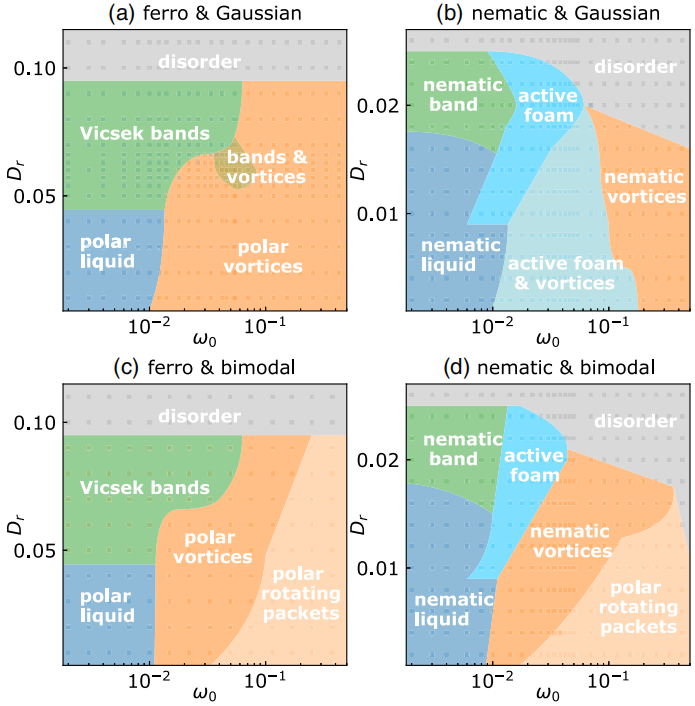
\includegraphics[width=0.49\textwidth]{./figs/capPhaseDiagram.png}
    \caption{
        \label{fig:capPhaseDiagram} Phase diagrams in the $\omega_0-D_r$ parameter space for the system \eqref{eq:CAPextension}.
        Reproduced with permission from ref.~\cite{PhysRevLett.127.238001}. Copyright 2021 American Physical Society.
    }
\end{figure}

\section{\label{sec:conclusions}Conclusions And Outlook}
In this review, we have discussed the collective behaviors of active matter, with a particular emphasis on the role of chemotaxis and chirality in shaping these behaviors. Chemotaxis is the ability of cells or organisms to move in response to chemical gradients in their environment, and it plays a crucial role in many biological processes, such as wound healing, immune response, and cancer metastasis. Chirality refers to the property of an object that is not superimposable on its mirror image, and it is a common feature of many biological systems, such as DNA, proteins, and cells. The combination of chemotaxis and chirality can lead to a wide range of interesting collective behaviors in active matter, such as phase separation, pattern formation, and dynamic self-assembly.

We have introduced the Keller--Segel and phoretic Brownian particle models of chemotactic active matter and discussed the role of chemotaxis in shaping the collective behaviors of active particles. We have presented the chiral active particle model and its extension and discussed the role of chirality in shaping the collective behaviors of active particles. Furthermore, we have summarized the main findings of the review and discussed future research directions in the field of active matter.

In the future, it would be interesting to investigate the role of chemotaxis and chirality in shaping the collective behaviors of active matter in more detail. For example, one could study the effects of different types of chemo-attractants on the collective behaviors of active particles and explore the role of chirality in shaping the collective behaviors of active particles. Furthermore, one could investigate the effects of different types of interactions between active particles on their collective behaviors and explore the role of external fields in shaping the collective behaviors of active particles. These studies could provide new insights into the fundamental principles governing the collective behaviors of active matter and could have important implications for the design of new materials and technologies based on active matter.

\begin{acknowledgments}
This work is partially supported by The Nonlinear Dynamics Research Group led by Professor Zheng and Institute of Systems Science, Huaqiao University, Xiamen.
\end{acknowledgments}

\bibliography{ref}

\end{document}
